\section*{\RU{Предисловие}\EN{Preface}\PTBRph{}\ESph{}\PLph{}}

\iffalse
\RU{Здесь (будет) немного моих заметок о \gls{reverse engineering} на русском языке для начинающих, 
для тех кто хочет научиться понимать создаваемый \CCpp компиляторами код для x86 (коего, 
практически, больше всего остального) и ARM.}
\EN{Here are some of my notes in English for beginners in \gls{reverse engineering}
who would like to learn to understand x86 (which accounts for almost
all executable software in the world) and ARM code created by \CCpp compilers.}
\fi

\RU{У термина \q{\gls{reverse engineering}} несколько популярных значений:
1) исследование скомпилированных
программ; 2) сканирование трехмерной модели для последующего копирования;
3) восстановление структуры СУБД. Настоящий сборник заметок
связан с первым значением.}
\EN{There are several popular meanings of the term \q{\gls{reverse engineering}}:
1) The reverse engineering of software: researching compiled programs;
2) The scanning of 3D structures and the subsequent digital manipulation required order to duplicate them;
3) recreating \ac{DBMS} structure.
This book is about the first meaning.}

\ifx\LITE\undefined
\subsection*{\RU{Рассмотренные темы}\EN{Topics discussed in-depth}\PTBRph{}\ESph{}\PLph{}}

x86/x64, ARM/ARM64, MIPS, Java/JVM.

\subsection*{\RU{Затронутые темы}\EN{Topics touched upon}\PTBRph{}\ESph{}\PLph{}}

\oracle (\myref{oracle}),
Itanium (\myref{itanium}),
\RU{донглы для защиты от копирования}\EN{copy-protection dongles} (\myref{dongles}), 
LD\_PRELOAD (\myref{ld_preload}),
\RU{переполнение стека}\EN{stack overflow}, 
\ac{ELF},
\RU{формат файла PE в win32}\EN{win32 PE file format} (\myref{win32_pe}),
x86-64 (\myref{x86-64}),
\RU{критические секции}\EN{critical sections} (\myref{critical_sections}),
\RU{системные вызовы}\EN{syscalls} (\myref{syscalls}), 
\ac{TLS},
\RU{адресно-независимый код}\EN{position-independent code} (\ac{PIC}) (\myref{sec:PIC}), 
profile-guided optimization (\myref{PGO}),
C++ STL (\myref{cpp_STL}),
OpenMP (\myref{openmp}),
SEH (\myref{sec:SEH}).
\fi

\subsection*{\RU{Об авторе}\EN{About the author}\PTBRph{}\ESph{}\PLph{}}

\begin{tabularx}{\textwidth}{ l X }

\raisebox{-\totalheight}{
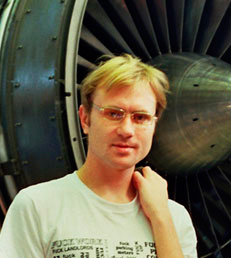
\includegraphics[scale=0.60]{Dennis_Yurichev.jpg}
}

&
\RU{Денис Юричев~--- опытный reverse engineer и программист.}%
\EN{Dennis Yurichev is an experienced reverse engineer and programmer.}
\EN{He can be contacted by email:}%
\RU{С ним можно контактировать по емейлу:} \textbf{\EMAIL{}}, 
\EN{or on Skype:}\RU{или по Skype:} \textbf{dennis.yurichev}.

% FIXME: no link. \tablefootnote doesn't work
\end{tabularx}

% subsections:
\subsection*{\RU{Отзывы о книге}\EN{Praise for} \IT{\TITLE}}

\begin{itemize}
% expanded URLs to make it more robust for printouts. In electronic editions people will click anyway, so tracking will keep working
\item \q{It's very well done .. and for free .. amazing.}\footnote{\href{http://go.yurichev.com/17095}{twitter.com/daniel\_bilar/status/436578617221742593}} Daniel Bilar, Siege Technologies, LLC.

\item \q{... excellent and free}\footnote{\href{http://go.yurichev.com/17096}{twitter.com/petefinnigan/status/400551705797869568}} Pete Finnigan, \RU{гуру по безопасности }\oracle\EN{ security guru}.

\item \q{... book is interesting, great job!} Michael Sikorski, \RU{автор книги}\EN{author of} \IT{Practical Malware Analysis: The Hands-On Guide to Dissecting Malicious Software}.

\item \q{... my compliments for the very nice tutorial!} Herbert Bos, \RU{профессор университета}\EN{full professor at the} Vrije Universiteit Amsterdam, \RU{соавтор}\EN{co-author of} \IT{Modern Operating Systems (4th Edition)}.

\item \q{... It is amazing and unbelievable.} Luis Rocha, CISSP / ISSAP, Technical Manager, Network \& Information Security at Verizon Business.

\item \q{Thanks for the great work and your book.} Joris van de Vis, \RU{специалист по} SAP Netweaver \& Security\EN{ specialist}.

\item \q{... reasonable intro to some of the techniques.}\footnote{\href{http://go.yurichev.com/17099}{reddit}} Mike Stay, \RU{преподаватель в}\EN{teacher at the} Federal Law Enforcement Training Center, Georgia, US.

\item \q{I love this book! I have several students reading it at the moment, plan to use it in graduate course.}\footnote{\href{http://go.yurichev.com/17097}{twitter.com/sergeybratus/status/505590326560833536}} \EN{Sergey Bratus}\RU{Сергей Братусь}, Research Assistant Professor \RU{в отделе Computer Science}\EN{at the Computer Science Department} \RU{в}\EN{at} Dartmouth College

\item \q{Dennis @Yurichev has published an impressive (and free!) book on reverse engineering}\footnote{\href{http://go.yurichev.com/17098}{twitter.com/TanelPoder/status/524668104065159169}} Tanel Poder, \EN{Oracle RDBMS performance tuning expert}\RU{эксперт по настройке производительности Oracle RDBMS}.

\item \q{This book is some kind of Wikipedia to beginners...} Archer, Chinese Translator, IT Security Researcher.

\RU{\item \q{Прочел Вашу книгу~--- отличная работа, рекомендую на своих курсах студентам
в качестве учебного пособия}. Николай Ильин, преподаватель в ФТИ НТУУ \q{КПИ} и DefCon-UA}
\end{itemize}


\subsection*{\RU{Благодарности}\EN{Thanks}\PTBRph{}\ESph{}\PLph{}}

\RU{Тем, кто много помогал мне отвечая на массу вопросов}\EN{For patiently answering all my questions}:
\HERMIT, \RU{Слава \q{Avid} Казаков}\EN{Slava \q{Avid} Kazakov}.

\RU{Тем, кто присылал замечания об ошибках и неточностях}\EN{For sending me notes
about mistakes and inaccuracies}:
\RU{Станислав \q{Beaver} Бобрицкий, Александр Лысенко}%
\EN{Stanislav \q{Beaver} Bobrytskyy, Alexander Lysenko}, Shell Rocket, Zhu Ruijin, Changmin Heo.

\RU{Просто помогали разными способами}\EN{For helping me in other ways}:
\RU{Андрей Зубинский}\EN{Andrew Zubinski}, 
Arnaud Patard (rtp \RU{на}\EN{on} \#debian-arm IRC),
\EN{Aliaksandr Autayeu}\RU{Александр Автаев}.

\RU{Переводчикам на китайский язык}\EN{For translating the book into Simplified Chinese}: Antiy Labs (\href{http://antiy.cn}{antiy.cn}) \AndENRU Archer.

\RU{Переводчику на корейский язык}\EN{For translating the book into Korean}: Byungho Min.

\RU{Корректорам}\EN{For proofreading}:
\RU{Александр \q{Lstar} Черненький}\EN{Alexander \q{Lstar} Chernenkiy},
\RU{Владимир Ботов}\EN{Vladimir Botov},
\RU{Андрей Бражук}\EN{Andrei Brazhuk},
\RU{Марк}\EN{Mark} ``Logxen'' \RU{Купер}\EN{Cooper},
Yuan Jochen Kang, Mal Malakov, Lewis Porter, Jarle Thorsen.

\RU{Васил Колев сделал очень много исправлений и указал на многие ошибки.}
\EN{Vasil Kolev did a great amount of work in proofreading and correcting many mistakes.}

\RU{За иллюстрации и обложку: Андрей Нечаевский.}\EN{For illustrations and cover art: Andy Nechaevsky.}

\RU{И ещё всем тем на github.com кто присылал замечания и исправления.}
\EN{Thanks also to all the folks on github.com who have contributed notes and corrections.}

\RU{Было использовано множество пакетов \LaTeX. Их авторов я также хотел бы поблагодарить.}
\EN{Many \LaTeX\ packages were used: I would like to thank the authors as well.}

\subsubsection*{\RU{Жертвователи}\EN{Donors}}

\EN{Those who supported me during the time when I wrote significant part of the book:}%
\RU{Те, кто поддерживал меня во время написании этой книги:}

2 * Oleg Vygovsky (50+100 UAH), 
Daniel Bilar ($\$$50), 
James Truscott ($\$$4.5),
Luis Rocha ($\$$63), 
Joris van de Vis ($\$$127), 
Richard S Shultz ($\$$20), 
Jang Minchang ($\$$20), 
Shade Atlas (5 AUD), 
Yao Xiao ($\$$10),
Pawel Szczur (40 CHF), 
Justin Simms ($\$$20), 
Shawn the R0ck ($\$$27), 
Ki Chan Ahn ($\$$50), 
Triop AB (100 SEK), 
Ange Albertini (\euro{}10+50),
Sergey Lukianov (300 RUR), 
Ludvig Gislason (200 SEK), 
Gérard Labadie (\euro{}40), 
Sergey Volchkov (10 AUD),
Vankayala Vigneswararao ($\$$50),
Philippe Teuwen ($\$$4),
Martin Haeberli ($\$$10),
Victor Cazacov (\euro{}5),
Tobias Sturzenegger (10 CHF),
Sonny Thai ($\$$15),
Bayna AlZaabi ($\$$75),
Redfive B.V. (\euro{}25),
Joona Oskari Heikkilä (\euro{}5),
Marshall Bishop ($\$$50),
Nicolas Werner (\euro{}12),
Jeremy Brown ($\$$100),
Alexandre Borges ($\$$25),
Vladimir Dikovski (\euro{}50),
Jiarui Hong (100.00 SEK),
Jim Di (500 RUR),
Tan Vincent ($\$$30),
Sri Harsha Kandrakota (10 AUD),
Pillay Harish (10 SGD),
Timur Valiev (230 RUR),
Carlos Garcia Prado (\euro{}10),
Salikov Alexander (500 RUR),
Oliver Whitehouse (30 GBP),
Katy Moe ($\$$14),
Maxim Dyakonov ($\$$3),
Sebastian Aguilera (\euro{}20),
Hans-Martin Münch (\euro{}15),
Jarle Thorsen (100 NOK),
Vitaly Osipov ($\$$100),
Yuri Romanov (1000 RUR),
Aliaksandr Autayeu (\euro{}10),
Tudor Azoitei ($\$$40),
Z0vsky (\euro{}10),
Yu Dai ($\$$10). 

\RU{Огромное спасибо каждому!}\EN{Thanks a lot to every donor!}

% subsections
\subsection*{mini-\RU{ЧаВО}\EN{FAQ}}

\newcommand{\HACKINGMdURL}{https://github.com/dennis714/RE-for-beginners/blob/master/HACKING.md}
\newcommand{\FNURLREDDIT}{\footnote{\href{http://go.yurichev.com/17027}{reddit.com/r/ReverseEngineering/}}}

Q: \EN{Why should one learn assembly language these days?}\RU{Зачем в наше время нужно изучать язык ассемблера?}\\
A: \EN{Unless you are an \ac{OS} developer, you probably don't need to code in assembly\EMDASH{}modern compilers 
are much better at performing optimizations than humans}
\RU{Если вы не разработчик \ac{OS}, вам наверное не нужно писать на ассемблере:
современные компиляторы оптимизируют код намного лучше человека}%
\footnote{\RU{Очень хороший текст на эту тему}\EN{A very good text about this topic}: \cite{AgnerFog}}.
\EN{Also, modern \ac{CPU}s are very complex devices and assembly knowledge doesn't really help one to understand their internals.}
\RU{К тому же, современные \ac{CPU} это крайне сложные устройства и знание ассемблера вряд ли
поможет узнать их внутренности.}
\EN{That being said, there are at least two areas where a good understanding of assembly can be helpful: 
First and foremost, security/malware research. It is also a good way to gain a better understanding of your compiled code whilst debugging.}
\RU{Но все-таки остается по крайней мере две области, где знание ассемблера может хорошо
помочь:
1) исследование malware (\IT{зловредов}) с целью анализа; 2) лучшее понимание
вашего скомпилированного кода в процессе отладки.}
\EN{This book is therefore intended for those who want to understand assembly language rather 
than to code in it, which is why there are many examples of compiler output contained within.}
\RU{Таким образом, эта книга предназначена для тех, кто хочет скорее понимать ассемблер,
нежели писать на нем, и вот почему здесь масса примеров, связанных с результатами
работы компиляторов.}\\
\\
Q: \RU{Я кликнул на ссылку внутри PDF-документа, как теперь вернуться назад?}\EN{I clicked on a hyperlink inside a PDF-document, how do I go back?}\\
A: \RU{В Adobe Acrobat Reader нажмите сочетание Alt+LeftArrow.}\EN{In Adobe Acrobat Reader click Alt+LeftArrow.}\\
\\
\ifx\LITE\undefined
Q: \RU{Ваша книга слишком большая! Нет ли чего покороче?}\EN{Your book is huge! Is there anything shorter?}\\
A: \RU{Есть сокращенная lite-версия}\EN{There is shortened, lite version found here}: \url{http://beginners.re/\#lite}.\\
\\
\fi
Q: \RU{Я не могу понять, стоит ли мне заниматься reverse engineering-ом}\EN{I'm not sure if I should try to learn reverse engineering or not}.\\
A: \RU{Наверное, среднее время для освоения сокращенной LITE-версии\EMDASH{}1-2 месяца.}%
\EN{Perhaps, the average time to become familiar with the contents of the shortened LITE-version is 1-2 month(s).}\\
\\
Q: \RU{Могу ли я распечатать эту книгу? Использовать её для обучения?}\EN{May I print this book? Use it for teaching?}\\
A: \RU{Конечно, поэтому книга и лицензирована под лицензией Creative Commons.}\EN{Of course! That's why the book is licensed under the Creative Commons license.}
\EN{One might also want to build one's own version of book\EMDASH{}read \href{\HACKINGMdURL}{here} to find out more.}
\RU{Кто-то может захотеть скомпилировать свою собственную версию книги, читайте \href{\HACKINGMdURL}{здесь} об этом.}\\
\\
Q: \RU{Я хочу перевести вашу книгу на другой язык}\EN{I want to translate your book to some other language}.\\
A: \RU{Прочитайте}\EN{Read} \href{https://github.com/dennis714/RE-for-beginners/blob/master/Translation.md}{\RU{мою заметку для переводчиков}\EN{my note to translators}}.\\
\\
Q: \RU{Как можно найти работу reverse engineer-а}\EN{How does one get a job in reverse engineering}? \\
A: \RU{На reddit, посвященному RE\FNURLREDDIT, время от времени бывают hiring thread}
\EN{There are hiring threads that appear from time to time on reddit, devoted to RE\FNURLREDDIT}
(\href{http://go.yurichev.com/17333}{2013 Q3}, 
\href{http://go.yurichev.com/17334}{2014}).
\RU{Посмотрите там}\EN{Try looking there}.
\EN{A somewhat related hiring thread can be found in the \q{netsec} subreddit}\RU{В смежном субреддите \q{netsec} имеется похожий тред}:
\href{http://go.yurichev.com/17335}{2014 Q2}.\\
\\
\RU{Q: Куда пойти учиться в Украине?\\
A: \href{http://go.yurichev.com/17336}{НТУУ \q{КПИ}: \q{Аналіз програмного коду та бінарних вразливостей}};
\href{http://go.yurichev.com/17337}{факультативы}.\\
\\}
Q: \EN{I have a question}\RU{У меня есть вопрос}...\\
A: \EN{Send it to me by email}\RU{Напишите мне его емейлом} (\EMAIL).


\ifdefined\ebook
\RU{Это версия формата A5 для электронных читалок}\EN{This is the A5-format version for e-book readers}. 
\RU{Хотя, тут всё то же самое, но иллюстрации уменьшены и не очень хорошо читаемы}
\EN{Although the content is mostly the same, the illustrations are resized and probably not readable}. 
\EN{You may try to change scale in your e-book reader.}
\RU{Вы можете попробовать изменить масштаб в вашей читалке.}
\RU{Так или иначе, вы всегда можете посмотреть их в версии формата A4 здесь}
\EN{Otherwise, you can always view them in the A4-format version here}: \href{http://go.yurichev.com/17009}{beginners.re}.
\fi

% {\RU{Целевая аудитория}\EN{Target audience}}

\subsection*{\RU{О переводе на корейский язык}\EN{About the Korean translation}\PTBRph{}\ESph{}\PLph{}}

\EN{In January 2015, the Acorn publishing company (\href{http://www.acornpub.co.kr}{www.acornpub.co.kr}) in South Korea did a huge amount of work in translating and publishing 
my book (as it was in August 2014) into Korean.}
\RU{В январе 2015, издательство Acorn в Южной Корее сделало много работы в переводе 
и издании моей книги (по состоянию на август 2014) на корейский язык.}

\RU{Она теперь доступна на}\EN{It's now available at} 
\href{http://go.yurichev.com/17343}{\EN{their website}\RU{их сайте}}.

\iffalse
\begin{figure}[H]
\centering
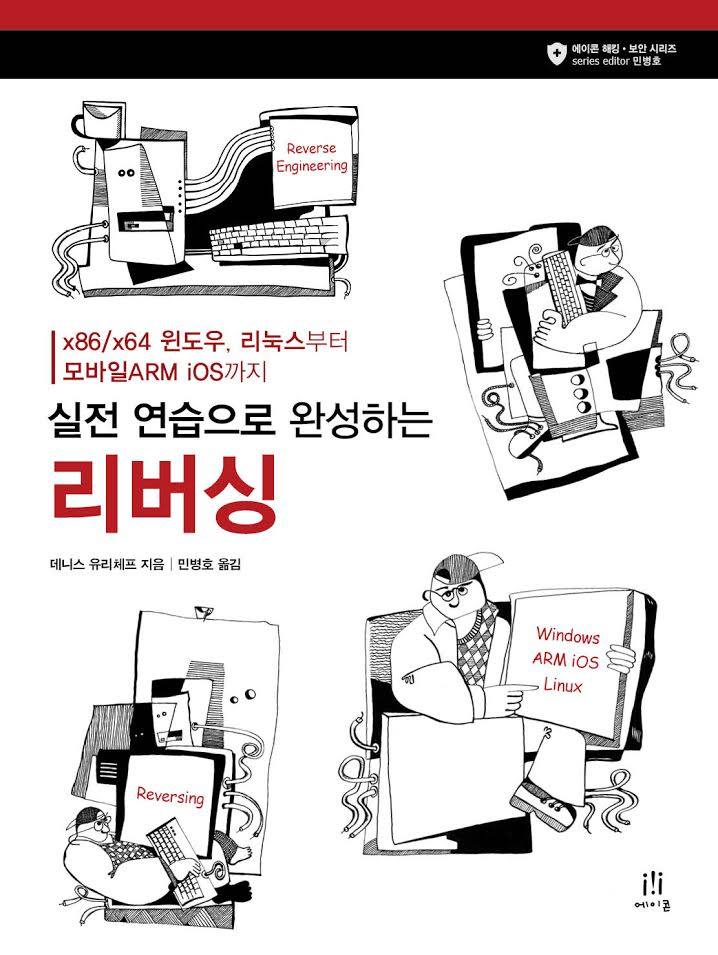
\includegraphics[scale=0.3]{acorn_cover.jpg}
\end{figure}
\fi

\RU{Переводил}\EN{The translator is} Byungho Min (\href{http://go.yurichev.com/17344}{twitter/tais9}).

\EN{The cover art was done by my artistic friend, Andy Nechaevsky}
\RU{Обложку нарисовал мой хороший знакомый художник Андрей Нечаевский}: 
\href{http://go.yurichev.com/17023}{facebook/andydinka}.

\RU{Они также имеют права на издании книги на корейском языке.}
\EN{They also hold the copyright to the Korean translation.}

\RU{Так что если вы хотите иметь \IT{настоящую} книгу на полке на корейском языке и
хотите поддержать мою работу, вы можете купить её.}
\EN{So, if you want to have a \IT{real} book on your shelf in Korean and 
want to support my work, it is now available for purchase.}
